\documentclass[12pt,listof=totoc]{scrartcl}

\usepackage{fancyhdr}
\usepackage{geometry}
\usepackage{ucs}
\usepackage[utf8x]{inputenc}
\usepackage[T1]{fontenc}
\usepackage[ngerman]{babel}
\usepackage{amsmath,amssymb,amstext}
\usepackage{hyperref}
\usepackage{cancel}
\usepackage{dsfont}
\usepackage{physics}
\usepackage{lmodern}
\usepackage{enumerate}
\usepackage{enumitem}
\usepackage{graphicx}
\usepackage{listings, color}
\usepackage[labelfont=bf]{caption}
\usepackage{titling}

\lstset{basicstyle=\scriptsize,breaklines=true} %Quellcode mit Umlauten und ganz klein
\lstset{literate=
  {Ö}{{\"O}}1
  {Ä}{{\"A}}1
  {Ü}{{\"U}}1
  {ß}{{\ss}}2
  {ü}{{\"u}}1
  {ä}{{\"a}}1
  {ö}{{\"o}}1
}


%Geometrie----------------------------------------------------------------------------------------------------------

\geometry{a4paper, top=25mm, left=15mm, right=15mm, bottom=25mm,headsep=10mm, footskip=10mm}
\pagestyle{fancy}
\setlength{\parindent}{0pt} %Zeileneinrückung

\fancyhf{} %Setzt voreingestellte Kopf-und Fußzeilen-Eigenschaften zurück

\lhead{\nouppercase{\leftmark}}
\chead{}
\rhead{\thepage}

\lfoot{}
\cfoot{}
\rfoot{}

\title{\vspace{0cm}{\Huge Fortgeschrittenen-Praktikum I:\\ \vspace{1cm} Szintillationszähler}}
\author{Saskia Bondza\\Simon Stephan}
\date{durchgeführt am 12.10.2016 und 13.10.2016}

\pretitle{%
  \begin{center}
  \LARGE
  
\includegraphics[width=6cm,]{figures/siegel}\\[\bigskipamount]
}
\posttitle{\end{center}}

%neue Commands----------------------------------------------------------------------------------------------------------
\newcommand{\nab}{\vec{\nabla}} %direkter Befehl mit Vektorpfeil
\newcommand{\gra}[3][0.7]{
	\begin{minipage}[h!]{\textwidth}
		\centering
		\includegraphics[width=#1\textwidth]{figures/#2.png}
		\captionof{figure}{#3}
	\end{minipage}
	\vskip 30 pt
}
\newcommand{\graShort}[4][0.7]{
	\begin{minipage}[h!]{\textwidth}
		\centering
		\includegraphics[width=#1\textwidth]{figures/#3.png}
		\captionof{figure}[#2]{#4}
	\end{minipage}
	\vskip 30 pt
}
\newcommand{\graTwo}[4][0.49]{
	\begin{minipage}[h!]{\textwidth}
		\centering
		\includegraphics[width=#1\textwidth]{figures/#2.png}
		\includegraphics[width=#1\textwidth]{figures/#3.png}
		\captionof{figure}{#4}
	\end{minipage}
	\vskip 30 pt
}
\newcommand{\graTwoShort}[5][0.49]{
	\begin{minipage}[h!]{\textwidth}
		\centering
		\includegraphics[width=#1\textwidth]{figures/#2.png}
		\includegraphics[width=#1\textwidth]{figures/#3.png}
		\captionof{figure}[#4]{#5}
	\end{minipage}
	\vskip 30 pt
}
\newcommand{\graTwoB}[5]{
	\begin{minipage}[h!]{\textwidth}
		\centering
		\includegraphics[width=#1\textwidth]{figures/#3.png}
		\includegraphics[width=#2\textwidth]{figures/#4.png}
		\captionof{figure}{#5}
	\end{minipage}
	\vskip 30 pt
}
\newcommand{\graThree}[5][0.49]{
	\begin{minipage}[h!]{\textwidth}
		\centering
		\includegraphics[width=#1\textwidth]{figures/#2.png}
		\includegraphics[width=#1\textwidth]{figures/#3.png}\newline
		\includegraphics[width=#1\textwidth]{figures/#4.png}
		\captionof{figure}{#5}
	\end{minipage}
	\vskip 30 pt
}
\newcommand{\del}[2][]{\frac{\partial #1}{\partial #2}}
\newcommand{\code}[1]{\texttt{#1}}


%Titel,Inhalt----------------------------------------------------------------------------------------------------------

\begin{document}
\pagenumbering{gobble} %verstecke Seitenzahl
\maketitle
\newpage

\section*{Abstract}

In diesem Versuch werden verschiedene $\gamma$-Strahler und ihre Wechselwirkung mit Materie untersucht wobei verschiedene Szintillatoren als Detektor verwendet werden. Ziel ist es dabei, ein Verständnis für die Funktionsweise von Szintillatoren zu entwickeln. Außerdem wird das Spektrum des Thorium-Isotops $^{228}Th$ aufgenommen  und die Winkelabhängigkeit der Paarvernichtung überprüft. Zusätzlich werden Spektren von Natriumproben unterschiedlichen Alters aufgenommen und ausgewertet.\\

In einem ersten Versuchsteil wurden mit einem NaI-Szintillationszähler die Zerfallsspektren von  $^{22}Na$, $^{60}Co$ und $^{152}Eu$ aufgenommen. Durch Identifizierung der bekannten Peaks aus den Zerfällen mit jeweils bekannten Energien haben wir dann eine Energiekalibrierung durchgeführt. Es wurde dann das Spektrum von $^{228}Th$ aufgenommen und die beobachteten Peaks mit Hilfe der zuvor durchgeführten Energiekalibrierung erfolgreich identifiziert. 
Die erwartete Winkelabhängigkeit mit einem Maximum bei 180° (gemessen: $\alpha_{max} = (181\pm 2)°$ konnte ebenfalls bestätigt werden.
Keine sinnvollen Ergebnisse erhielten wir jedoch bei der Untersuchung der Natriumproben unterschiedlichen Alters.

\newpage

\thispagestyle{empty}
\tableofcontents
\newpage

%Schreiben----------------------------------------------------------------------------------------------------------
\pagenumbering{arabic} %verstecke Seitenzahl
\section{Einleitung}



Zur Messung radioaktiver Spektren gibt es eine Reihe verschiedener Methoden. So kann beispielsweise ein Halbleiterdetektor oder ein Zählrohr verwendet werden, um radioaktive Zerfälle zu untersuchen (vgl. siehe Referenz \cite{staat} und \cite{staat1}). In diesem Versuch werden Szintillationszähler, die aus einem Szintillator und einem Photomultiplier bestehen, zur Untersuchung radioaktiver Proben und Aufnahme der Spektren verwendet. Hier wird Photoemission im Szintillator durch einfallende Strahlung hervorgerufen, die der Photomultiplier in ein Stromsignal umwandelt.

Es wird ein auf Grund seiner höheren Lichtausbeute für Energiemessungen besser geeigneter anorganischer NaI-Szintillator verwendet sowie ein auf Grund seiner schnelleren Abklingzeit für Zeitmessungen besser geeigneter organischer Plastikszintillator.
Zur Signalverarbeitung werden Geräte des NIM-Standards ("`Nuclear Instrument Module"') verwendet, der sich in der Teilchenphysik bewährt hat.\\

Der Versuch ist in drei Teile untergliedert. 
In einem ersten Versuchsteil wird mit dem energiesensiblen NaI-Szintillationszähler das Spektrum von $^{228}Th$ aufgenommen und die Peaks identifiziert, wofür zunächst eine Energiekalibrierung durchgeführt werden muss. Diese wird an Hand von Spektren von  $^{22}Na$, $^{60}Co$ und $^{152}Eu$ und der bekannten Peaks durchgeführt.
Im zweiten Teil des Versuchs wird die Winkelabhängigkeit der beim $\beta^{+}$-Zerfall in $^{22}Na$ auftretenden Photonen, die durch Paarvernichtung entstehen, untersucht. Hier werden beide Szintillatoren verwendet, wobei der Plastikszintillator auf einem drehbaren Arm montiert ist, sodass der Winkel zwischen beiden Szintillatoren verstellbar ist. Es werden Messungen der Koinzidenzen bei verschiedenen Winkeln vorgenommen.
Im dritten Teil des Versuchs werden die Spektren von Natriumproben unterschiedlichen Alters aufgenommen und mit Datensätzen aus anderen Jahren verglichen.
Beim Optimieren der Einstellungen und besseren Verständnis der einzelnen Geräte half ein Oszilloskop, auf dem die Signale beobachtet wurden.



\newpage
\section{Theoretische Grundlagen}

Dieser Abschnitt orientiert sich im Wesentlichen an Referenz \cite{staat}. Es werden die für das Verständnis dieses Versuches wesentlichen Hintergründe erklärt. 

\subsection{Zerfallsgesetz\label{zerfallsgesetz}}
Der radioaktive Zerfall ist ein statistischer Prozess, d.h. der genaue Zeitpunkt, zu dem ein Kern zerfällt, kann nicht vorhergesagt werden. Wir können nur Wahrscheinlichkeiten angeben. Die Zerfallsrate $\frac{dN}{dt}$ ist abhängig von der momentanen Anzahl $N$ der Atome.
\[\frac{dN}{dt}=-\lambda N\]
wobei $\lambda$ die Zerfallskonstante ist, welche den Bruchteil der zu Beginn vorhandenen Kerne, die pro Zeiteinheit zerfallen, beschreibt\textsuperscript{\cite{Demtröder}}. Kann ein Kern auf verschiedene Arten zerfallen, so addieren sich die Zerfallskonstanten der einzelnen Zerfallsprozesse. Durch Lösen der obigen Differentialgleichung erhält man die Anzahl der Kerne $N$ zum Zeitpunkt $t$:
\[N(t)=N_0e^{-\lambda t}\hspace{0.5cm}\]
wobei $N_0=N(t=0)$ die anfängliche Anzahl der Kerne beschreibt. Hieraus lässt sich dann die mittlere Lebensdauer $\tau$ bestimmen:
\[\tau=\frac{1}{\lambda}\]
welche mit der Halbwertszeit $T_{1/2}$ wie folgt zusammenhängt:\textsuperscript{\cite{Demtröder}}
\[T_{1/2} = \ln2\cdot \tau = \frac{\ln2}{\lambda}\]
 


\subsection{Radioaktive Zerfälle}
In diesem Versuch werden verschiedene radioaktive Proben untersucht, die auf unterschiedliche Weise zerfallen.
Instabile Atomkerne gehen, je nach Art des Zerfalls, unter Aussendung von ionisierender Strahlung und Aussendung von Teilchen spontan in einen anderen Atomkern über. Im Folgenden werden die verschiedenen Arten radioaktiver Zerfälle erläutert.
\subsubsection{$\alpha$-Zerfall}
Beim $\alpha$-Zerfall geht ein schwerer, instabiler Kern unter Aussendung eines $\alpha$-Teilchens, einem Heliumkern (zwei Protonen und zwei Neutronen) in einen stabilen Kern über. Die Massenzahl des neuen Atomkerns ist dabei um vier gesunken, die Ordnungszahl verringert sich um zwei.\textsuperscript{\cite{Demtröder}}

\begin{align}
{}_Z^A X \rightarrow {}_{Z-2}^{A-4} Y + {}^4_2He
\end{align}

\subsubsection{$\beta$-Zerfall \label{beta}}
Der $\beta$-Zerfall wird durch verschiedene Prozesse der schwachen Wechselwirkung beschrieben bei denen Elektronen  und Positronen auftreten. Bei diesem Vorgang wird durch W-Boson-Austausch ein Proton in ein Neutron umgewandelt bzw. ein Neutron in ein Proton.\textsuperscript{\cite{Demtröder}}

\paragraph*{$\beta^-$-Zerfall:} 
Bei dieser Art des Zerfalls wandelt sich ein Neutron im Kern unter Aussendung eines Elektrons und eines Elektron-Antineutrinos in ein Proton um. 
\begin{align*}
n &\rightarrow p + e^- + \bar{\nu_e}\\
{}_Z^A X &\rightarrow {}_{Z+1}^A Y + e^- + \bar{\nu_e}
\end{align*}

Hierbei entspricht X dem Mutternuklid und Y dem Tochternuklid. Die Ordnungszahl erhöht sich bei diesem Vorgang um eine Einheit, die Massenzahl ändert sich nicht.

\paragraph*{$\beta^+$-Zerfall:}
Der $\beta^+$-Zerfall ist dem $\beta^-$-Zerfall sehr ähnlich, Hier wandelt sich ein Proton im Kern unter Aussendung eines Positrons und eines Elektron-Neutrinos in ein Neutron um.
\begin{align*}
p &\rightarrow n + e^+ + \nu_e\\
{}_Z^A X &\rightarrow {}_{Z-1}^A Y + e^+ + \nu_e
\end{align*}

Bei diesem Prozess sinkt die Kernladungszahl um eine Einheit während die Massenzahl wie auch beim $\beta^-$-Zerfall unverändert bleibt.

\subsubsection{Elektroneneinfang}
Die meisten schweren, instabilen Kerne mit Protonenüberschuss wandeln sich durch Elektroneneinfang in stabile Kerne um.
Der Elektroneneinfang führt effektiv im Kern zum gleichen Resultat wie der $\beta^+$-Zerfall, d.h. die Ordnungszahl verringert sich um eine Einheit, die Massenzahl bleibt unverändert. Meist wird aus der Kern-nächsten Schale, der K-Schale, ein Bahnelektron unter Aussendung eines Neutrinos eingefangen. Die Lücke, die hierbei entsteht, wird meist durch ein aus der L-Schale stammendes Elektron unter Emission von Röntgenstrahlung oder Auger-Elektronen (siehe \ref{auger}) gefüllt. Dieser Vorgang wiederholt sich mit den weiter außen liegenden Schalen.
\[{}_Z^A X + e^- \rightarrow\ {}_{Z-1}^A Y + \nu_e\]
\subsubsection{$\gamma$-Zerfall \label{gamma}}

Der $\gamma$-Zerfall ist oft eine Begleiterscheinung der bereits diskutierten Kernzerfälle: Befindet sich das Tochternuklid nach dem Zerfall in einem angeregten Zustand, geht es über Aussendung eines $\gamma$-Quants (Photon) in einen energetisch niedrigeren Zustand über. Die Energie dieser Photonen liegt dabei im Bereich von keV bis MeV. In Materie fällt die Intensität $I_d$ der $\gamma$-Strahlung exponentiell mit der Strecke $d$ ab:
\[I_d=I_0e^{-\mu d}\]
Dabei ist $\mu$ der Absorptionskoeffizient des Materials und $I_0$ die Anfangsintensität.\textsuperscript{\cite{Demtröder}}

%\subsubsection{Innere Konversion}
%Konkurrierend zum $\gamma$-Zerfall gibt es auch die Innere Konversion. Bei dieser gehen angeregte Kernzustände strahlungslos in den Grundzustand über, wobei die Energie an ein Elektron übertragen und dieses abgestrahlt wird. Die so entstandene Lücke in der Atomhülle wird dann unter Emission von Röntgenstrahlung oder Auger-Elektronen (siehe \ref{auger}) gefüllt.\textsuperscript{\cite{anleitung1}}
%
%\subsection{Prozesse in der Atomhülle}\label{auger}
%Bei manchen Zerfallsprozessen entsteht in der Atomhülle durch Emission eines Elektrons ein Loch. Dieses Loch wird gefüllt, indem ein Elektron einer höheren Schale in die Schale des Loches wechselt und dabei Energie freigibt. Diese Energie kann entweder über direkte Emission eines Photons (Röntgenstrahlung) oder über die Emission eines anderen Elektrons (Auger-Elektron) abgegeben werden. Dadurch entstehen ein oder zwei neue Lücken, welche wiederum über die weitere Emission von Röntgenstrahlung oder eines Auger-Elektrons geschlossen werden können.\textsuperscript{\cite{anleitung1}}

\subsection{Wechselwirkung von $\gamma$-Strahlung mit Materie}
Um $\gamma$-Strahlung detektieren zu können, muss die $\gamma$-Strahlung mit Materie wechselwirken. Wir unterscheiden dabei grundsätzlich drei Prozesse: Den Photoeffekt, den Compton-Effekt und die Paarbildung.
 \subsubsection{Photo-Effekt}
 Beim Photoeffekt dringt ein Photon in das Atom ein und überträgt seine gesamte Energie an ein Elektron der inneren Schalen. Dabei wird Energie auf dieses Elektron übertragen, es wird aus der Atomhülle befreit und erhält kinetische Energie. Die hier entstandene Lücke wird über Abstrahlung eines $\gamma$-Quants oder eines Elektrons wieder gefüllt. Dies wird als äußerer Photoeffekt bezeichnet (siehe Abbildung \ref{PHOTO}) .

  \gra{Photo}{Äußerer Photoeffekt\cite{staat} \label{PHOTO}}
  Reicht die Energie des Photons nicht aus, um das Elektron zu befreien, wird es in eine höhere Schale angeregt. Dies wird als innerer Photoeffekt bezeichnet.
  Der Photoeffekt findet typischerweise bei Energien bis zu $200$ keV statt.\textsuperscript{\cite{anleitung1}}
 \subsubsection{Compton-Effekt}
 Beim Compton-Effekt trifft ein einfallendes $\gamma$-Quant auf ein freies oder nur leicht gebundenes Elektron und überträgt einen Teil seiner Energie auf dieses. Dieser Prozess findet meist bei Energien zwischen $200$ keV und $5$ MeV statt.\textsuperscript{\cite{anleitung1}}
 

 \graShort{Compton-Effekt}{Compton}{links: In dieser Darstellung kann man ein Photon sehen, das mittels Comptoneffekt an einem Elektron gestreut wird und dabei Energie verliert, da es nach dem Stoß langwelliger ist.\cite{staat} rechts: Dieser Graph skizziert den erwarteten Verlauf im Energiespektrum einer einzelnen
 Photonenenergie durch Compton- und Photoeffekt. Die Wölbung des Comptonplateaus ist nicht zu
 sehen.\cite{med}}
 \subsubsection{Paarbildung und Paarvernichtung \label{PVN1}}
 Bei der Paarbildung entsteht durch die Wechselwirkung des $\gamma$-Quants mit dem elektromagnetischen Feld des Atomkerns oder eines Elektrons ein Teilchen-Antiteilchen-Paar, z.B. Elektronen-Positronen-Paar. Paarbildung ist für Energien über $1,022$ MeV möglich. Die über diesen Grenzwert hinausgehende Energie wird auf die entstandenen Teilchen übertragen, der Impuls wird vom Kern aufgenommen. Da das Positron nicht lange alleine existieren kann, vereinigt es sich unter Abstrahlung von zwei $\gamma$-Quanten mit einer Energie von je 511 keV mit einem Elektron. Auf Grund der Impulserhaltung wird für die beiden $\gamma$-Quanten ein Winkel von 180° erwartet. \textsuperscript{\cite{anleitung}}

 
 \subsection{Zerfallsreihen der verwendeten Präparate \label{ZR}}
 
 Das Produkt eines radioaktiven Zerfalls kann instabil sein und ebenfalls zerfallen. Diese
 Abfolge von Zerfällen wird Zerfallsreihe genannt. Nachfolgend werden die Zerfallsreihen der verwendeten radioaktiven Isotope und die sich hieraus ergebenden erwarteten Peaks im Spektrum erläutert.
 
 \subsubsection{Natrium $^{22}Na$}
 Das in diesem Versuch verwendete Natrium-Isotop $^{22}Na$ zerfällt mit einer Halbwertszeit von $T=2,6088$ Jahren zu  89,9\% durch $\beta^+$ -Zerfall und zu  10,1 \% durch Electron Capture (siehe Abschnitt \ref{beta}) und zu  in den angeregten Kernzustand 2+ von $^{22}Ne$. Die Zerfallsreihe ist in Abbildung \ref{NA} dargestellt. Bei beiden Zerfällen entstehen Positronen, die in Materie mit Elektronen annihilieren und dabei zwei $\gamma$-Quanten mit einer Energie von $511\,\mathrm{keV}$ abstrahlen (siehe Abschnitt \ref{PVN1}). Da Impulserhaltung gilt, erwartet man für diese einen Winkel von $180\,\mathrm{°}$. Die Winkelabhängigkeit wird in \ref{WdP} überprüft. Man erwartet im Natriumspektrum also einen Peak von $511\,\mathrm{keV}$. Zusätzlich erwartet man einen Peak bei $1274,6\,\mathrm{keV}$, dies entspricht der Energie des Photons, das beim Übergang in den Grundzustand frei wird (siehe Abschnitt \ref{gamma}).\textsuperscript{\cite{staat}}. Das von uns gemessene Natriumspektrum ist in \ref{natriumbild} dargestellt.
 
 \gra{Zerfallsreihe-Na}{Zerfallsreihe von $^{22}Na$ \label{NA} \cite{staat}}
 
 \subsubsection{Cobalt  $^{60}Co$}
 $^{60}Co$ zerfällt durch zwei $\beta^-$ -Zerfälle mit annähernd 100 \% in den angeregten Zustand 4+ von  $^{60}Ni$, wobei die Halbwertszeit $T=5,2714$ Jahre beträgt. Die höchste Wahrscheinlichkeit hat dann der Übergang vom 4+ in den 2+ Kernzustand. Im Energiespektrum von $^{60}Co$ sind somit Peaks bei $1173,2$ keV und $1332,5$ keV  zu erwarten, wobei ersterer der Energiedifferenz zwischen dem 4+ und dem 2+ Kernzustand entspricht und der zweite der Energiedifferenz des Übergangs in den Grundzustand\textsuperscript{\cite{staat}} (siehe Abbildung \ref{Co} ). Das von uns gemessene Cobaltspektrum ist in Abbildung \ref{cobaltbild} dargestellt.
 
 \gra{Zerfallsreihe-Co}{Zerfallsreihe von $^{60}Co$ \label{Co} \cite{staat} }
 
 \subsubsection{Europium  $^{152}Eu$}
 Das Europium Isotop $^{152}Eu$ zerfällt mit einer Halbwertszeit von 12 Jahren durch $\beta^-$ -Zerfall in   $^{152}_{64}Gd$ sowie $\beta^+$ -Zerfall und Electron Capture in $^{152}_{62}Sm$. Der Übergang der angeregten Zustände von  $^{152}_{64}Gd$ und $^{152}_{62}Sm$ in den Grundzustand entspricht Peaks bei 122 keV und 344 keV. In Abbildung \ref{Eu} sind die für diesen Versuch relevanten Zerfälle dargestellt.\textsuperscript{\cite{staat}}. Das von uns gemessene Europiumspektrum ist in Abbildung \ref{europiumbild} dargestellt.
 
 
 \gra{Zerfallsreihe-Eu}{Vereinfachte Zerfallsreihe von $^{152}Eu$ \label{Eu} \cite{staat}}
 
  \subsubsection{Thorium  $^{228}Th$}
  In Abbildung \ref{Th} ist die Zerfallsreihe von Thorium  $^{232}Th$ dargestellt, die $^{228}Th$ als Zerfallsprodukt enthält. Es wird hier auf Grund der Komplexität dieser Zerfallsreihe auf die Darstellung der wahrscheinlichsten Übergänge und deren zugehörigen Peaks verzichtet und Referenz \cite{staat} verwiesen. Das von uns gemessene Thoriumspektrum ist in Abbildung \ref{thoriumGes} dargestellt.
  
  \gra{Zerfallsreihe-Th}{Zerfallsreihe von  $^{228}Th$ \label{Th} \cite{staat}}
 
 
 
 \subsection{Szintillationszähler \label{SZ}}
 
 In diesem Versuch werden Szintillationszähler als Detektoren verwendet.
 Ein Szintillationszähler besteht aus einem Szintillator und einem Photomultiplier, die in diesem Versuch mit dem Vorverstärker in einem Gehäuse sind, um Kabelwege zu reduzieren und damit Rauschen und Störsignale zu vermeiden.
 In Abbildung \ref{Szintiyay} ist die Funktionsweise eines Szintillators dargestellt.Mit Szintillatoren bezeichnet man spezielle Messgeräte, mit denen hochenergetische Photonen in Strahlung niedrigerer Energie aber höherer Intensität umgewandelt werden. Die Intensität der Szintillatorstrahlung ist proportional zur Energie der zu detektierenden Strahlung. Im Szintillationsmedium regt die radioaktive Strahlung durch Kernprozesse die Emission von Photonen an. Diese Photonen können das Medium durchdringen und werden in einem Photomultiplier verstärkt und gemessen. Die Funktionsweise eines Photomultipliers kann in Referenz \cite{Demtröder} nachgelesen werden.

 \gra{Szinti}{Funktionsweise eines Szintillationszählers \cite{Demtröder} \label{Szintiyay} }
 
 In diesem Versuch wird ein organischer Plastikszintillator sowie ein anorganischer NaI-Szintillator verwendet. 
 
 \subsubsection{Organischer Szintillator \label{OSZ}}
 
 Organische Szintillatoren haben den Vorteil, dass sie auf Grund der geringeren Abklingzeit eine bessere Reaktionszeit haben und sich somit gut für Zeitmessungen eignen. Der in diesem Versuch verwendete Plastikszintillator besteht aus einer Trägersubstanz und einer Aktivatorsubstanz. Einfallende Photonen regen die Moleküle des Plastikmaterials an, die ihre Energie dann auf die Moleküle der Aktivatorsubstanz übertragen. Die Moleküle der verschiedenen Stoffe haben dabei unterschiedliche Energieniveaus. Beim Abregen der Moleküle der Aktivatorsubstanz werden Photonen der gleichen Energie emittiert, die den Szintillator verlassen und vom Photomultiplier detektiert werden können.
 Das Outputsignal des Plastikszintillationszählers nach dem Vorverstärker ist in Abbildung \ref{soidgj} dargestellt. Es hat eine Breite von einigen hundert Nanosekunden.\textsuperscript{\cite{staat}}
 
 \vskip 10 pt
  \graShort[0.5]{Outputsignal eines Plastikszintillators}{Plastik-Szinti}{Das Outputsignal des Plastikszintillators nach dem Vorverstärker auf dem gelben Kanal  \label{soidgj}}

 \subsubsection{Anorganischer Szintillator \label{ASZ}}
 
 Anorganische Szintillatoren haben eine deutlich bessere Energieauflösung als organische Szintillatoren. Dies liegt an ihrer hohen Ordnungszahl und Dichte die eine hohe Nachweiswahrscheinlichkeit mit sich bringt. Der in diesem Versuch verwendete NaI-Kristall ist mit Thalium dotiert. 
 Dringen Photonen in den Kristall ein, können sie ihre Energie durch Photo-bzw. Comptoneffekt an die Elektronen im Valenzband übertragen, die dann in das Leiterband angeregt werden können. Diese regen sich dann unter Aussendung eines niederenergetischen Photons wieder ab und fallen in das Valenzband zurück. Eine Dotierung mit Thalium verhindert durch zusätzliche Energieniveaus zwischen Valenz-und Leitungsband in die Elektronen aufgenommen werden können, eine ständige Reabsorption und Emission der Photonen, sodass diese den Kristall verlassen und detektiert werden können.
 
  \graShort[0.5]{Outputsignal eines NaI-szintillationszählers}{NaI-Szinti}{Das Outputsignal des NaI-Szintillationszählers nach Vorverstärker auf dem gelben Kanal \label{GO}}
  
  In Abbildung \ref{GO} ist das Outputsignal des im Versuch verwendeten NaI-Szintillationszählers nach Vorverstärker zu sehen. Die Breite des Signals ist hier in der Größenordnung von ca, 50 Mikrosekunden, und damit deutlich breiter als das Signal des Plastikszintillationszählers (siehe Abbildung \ref{soidgj}). Die erwartete höhere Lichtausbeute ist durch die deutlich größere Fläche der Kurve ebenfalls bestätigt.\textsuperscript{\cite{staat}}
 \subsection{Gerätebeschreibung \label{Geräte}}
 
 Die verschiedenen Geräte, die im Versuchsaufbau als Teil der NIM-Module verwendet werden, sind im Folgenden aufgelistet und ihre Funktionsweise wird erklärt:
 
 \paragraph{Detektor} Der Szintillator und der Photomultiplier bilden zusammen den Detektor.
 \paragraph{Vorverstärker}
 Der Vorverstärker (VV) verstärkt die schwachen Signale des Detektors und verbessert so
 das Signal zu Rausch Verhältnis. Um Signalverluste entlang der Kabel zu reduzieren, ist der PA im Gehäuse des PM integriert. Die Pulsform des Ausgangssignals besitzt eine negative Amplitude und nimmt exponentiell zu.
 \paragraph{Hauptverstärker (HV)}
 Der Hauptverstärker  verstärkt das Spannungssignal rauscharm und erzeugt einen möglichst kurzen Puls, dessen Dauer Amplituden-unabhängig ist. Die Pulshöhe ist dabei annähernd proportional zur deponierten Ladungsmenge im Szintillator. Der Hauptverstärker hat zwei verschiedene Ausgänge, die entweder ein bipolares Signal (zeitsensible Messungen) oder ein unipolares Signal (Aufnahme der Spektren) liefern.
 
 \graTwoShort[0.5]{Plastik-Verstaerker}{NaI-Verstaerker}{Signale vor und nach Hauptversärker}{oben:Plastik-szintillationszähler unten: NaI-Szintillationszähler; Kanal 1: Signal nach dem VV Kanal 2: Unipolarer Ausgang des HV Kanal 3: Bipolarer Ausgang des HV \label{HV}}
 
 In Abbildung \ref{HV} sind die Signale der verwendeten Szintillationszähler je vor dem HV (nach dem VV) und die beiden Outputsignale des HV dargestellt.
 \paragraph{Multi Channel Analyser (MCA)}
 Der Multi Channel Analyser ordnet jeden eingehenden Puls, abhängig von der Pulshöhe (also von der im Szintillator deponierten Ladungsmenge), einem Channel zu. Das so erhaltene Energiespektrum kann als Histogramm dargestellt werden.
 \paragraph{Single Channel Analyser (SCA)}
 Ein Single Channel Analyser selektiert aus eingehenden Signalen in dem nur für Energien in einem einstellbaren Energiefenster ein Ausgangspuls erzeugt wird.  Für die Messung der Koinzidenzen soll hier das Energiefenster so eingestellt werden, dass möglichst nur Signale des 511 keV Peak weitergegeben werden.
 \paragraph{Gate} Das Gate hat zwei Eingänge. Sofern am Enable-Eingang ein Signal ankommt, wird das Signal des anderen Eingangs während dieser Zeit direkt als Output weitergeleitet. Die Dauer des Gatesignals kann mit einem Schlitzschraubenzieher eingestellt werden.
 \paragraph{Timing Unit}
 In der Timing Unit werden negative logische Signale verarbeitet und daraus ein rechteckiges Ausgangssignal erzeugt, dessen Breite sich mit Hilfe eines Schlitzschraubenziehers einstellen lässt.
 \paragraph{Coincidence Unit}
 Man spricht von einer Koinzidenz wenn zwei oder mehr Signale zeitgleich auftreten. Sofern eine Koinzidenz (dies kann durch Überschreiten einer Schwelle von der Summe beider Signale erfasst werden) vorliegt, erzeugt die Koinzidenzeinheit ein logisches Ausgangssignal.
 \paragraph{HEX Counter}
Der HEX-Counter zählt die eintreffenden Signale sowie die Zeit.

\subsection{Energiespektrum}\label{saskiascoolerabschnitt}

Das Energiespektrum, das aus den gemessenen Photonenenergien entsteht, weist  charakteristische Merkmale auf. Diese sind im Folgenden erklärt. 
 
 
 \paragraph{Photopeak}
 
 Wird die gesamte Energie eines von der Quelle stammenden Photons im Szintillator absorbiert, so wird dies im Spektrum einem Photopeak zugeordnet. Die zu erwarteten Photopeaks sind vom Präparat abhängig und sind in Kapitel \ref{ZR} erklärt.
 \paragraph{Escape-Peak}
 Wenn ein Röntgenquant den Szintillator ohne Wechselwirkung verlassen kann, folgt ein Verlust der Differenz der Bindungsenergie zwischen K-, und L-Schale. Diese Differenz beträgt im Fall des NaI-Szintillators $28$ keV. Damit sind Escapepeaks bei $E_\gamma - 28$ keV zu erwarten, wobei $E_\gamma$ die Energie eines Photopeaks ist.

 \paragraph{Compton-Kante}
 Die maximale Energie, die ein Photon durch den Compton-Effekt auf ein Elektron übertragen kann, entspricht im Spektrum der Compton-Kante. Diese ist charakterisiert durch einen starken Abfall der Zählrate.
 
 \paragraph{Rückstreupeak}
 
 Die Rückstreuung unter einem Winkel von 180 ° hat beim Compton-Effekt die höchste Wahrscheinlichkeit.
 Man beobachtet daher einen Rückstreu-Peak im Spektrum unterhalb der Compton-Kante.

 
 \paragraph{Röntgen-Fluoreszenz-Peak}
Es können in der Quelle Wechselwirkungen von $\gamma$-Quanten mit Elektronen stattfinden, ohne dass diese vom Szintillator detektiert werden. Geht ein Elektron von einer höheren Schale in jene Schale über aus der ein Elektron ausgetreten ist, kann ein Auger-Elektron oder charakteristische Röntgenstrahlung freigesetzt werden. Die Energie dieser charakteristischen Röntgenstrahlung ist dann als Röntgen-Fluoreszenz-Peak im Energiespektrum zu beobachten.




\newpage
\section{Versuchsaufbau und -Durchführung}

Nachfolgend ist der Versuchsaufbau für die verschiedenen Teile des Versuchs erklärt sowie die Versuchsdurchführung protokolliert. Zur Optimierung der Einstellungen und Überprüfen der Signale wurde ein Oszilloskop verwendet. Da dieses keinen der zur Verfügung stehenden USB-Sticks erkannte, wurden mit dem Handy Fotos gemacht. Diese wurden anschließend mit dem Programm \code{GIMP} nachbearbeitet.

\subsection{Teil I: Vorbereitung und Energiekalibrierung \label{Teil1}}

\gra[0.9]{schaltbild1}{Versuchsaufbau zur Aufnahme der Energiespektren \label{SB1}}


Die für die Aufnahme der Spektren verwendete Schaltung ist in Abbildung  \ref{SB1} dargestellt. Die Funktionsweise der einzelnen Geräte wird in \ref{Geräte} erklärt. Das Stromsignal des Photomultipliers wird zum Vorverstärker geleitet. Dessen Ouptput wird zum Hauptverstärker geleitet, dessen unipolarer Output an dem MCA weitergeleitet wird. Dieser ist mit einem Computer verbunden auf dem ein passendes Messprogramm installiert ist. Die erwarteten Signalformen aus den verschiedenen Ausgängen der Geräte sind in blau dargestellt.
Auf Grund der besseren Energieauflösung anorganischer Szintillatoren wird in diesem Versuchsteil  der NaI-Szintillator verwendet (siehe \ref{ASZ}). Die Probe wird in einem Bleiblock mit einer Öffnung in Richtung des Szintillators befestigt. \\

Das Signal wird zunächst nach dem Szintillator sowie nach den beiden Verstärkern betrachtet und die Einstellungen entsprechend optimiert. Die Verstärkung des Hauptverstärkers ist so einzustellen, dass die Channelzahl am MCA gut genutzt wird. Dabei ist zu berücksichtigen, dass die Einstellungen für die Aufnahme aller Spektren unverändert bleiben soll, sodass sicherzustellen ist, dass alle Peaks mit den gewählten Einstellungen gemessen werden können. Am Messprogramm des MCAs ist die Channelanzahl sinnvoll zu wählen, wir haben hier eine Channelanzahl von 8192 gewählt, um eine gute Energieauflösung mit ausreichend Counts zu erhalten. Außerdem wurden durch eine Einstellung des Messprogramms die ersten 0.2\% der Spektren abgeschnitten, da der MCA in diesem Bereich oftmals fehlerhafte Werte anzeigt. Die anderen gewählten Einstellungen können \ref{Laborbuch} entnommen werden.
Die Spektren von $^{22}Na$, $^{60}Co$ und $^{152}Eu$ werden jeweils 30 Minuten lang aufgenommen. Außerdem wird nach Entfernung der Probe aus dem Versuchsaufbau eine Untergrundmessung bei identischem Versuchsaufbau und mit einer Messzeit von drei Stunden durchgeführt. Das Spektrum von  $^{228}Th$ wird über Nacht aufgenommen.


\subsection{Teil II: Messung der Koinzedenzen}
In diesem Versuchsteil wird die Winkelabhängigkeit der Paarvernichtung untersucht. Dazu wird eine Natriumprobe verwendet und die Anzahl der Koinzidenzen in Abhängigkeit des Winkels gemessen.

\gra[0.95]{schaltbild2}{Versuchsaufbau zur Untersuchung der Winkelabhängigkeit \label{SB2}}

Der Versuchsaufbau und die verwendete Schaltung für diesen Versuchsteil kann Abbildung \ref{SB2} entnommen werden. Die Funktionsweise der Geräte wird in Kapitel \ref{Geräte} erklärt.  Die erwarteten Pulsformen sind in blau dargestellt. Der Plastikszintillator ist auf einem drehbaren Arm montiert, sodass der Winkel der beiden Szintillatoren zueinander verstellbar ist. In 5°-Schritten sind dabei Einkerbungen zu finden, die den Detektor einrasten lassen. Von den Szintillationszählern werden Signale wie zuvor über einen Vorverstärker zum Hauptverstärker geleitet. Der bipolare Ausgang des Hauptverstärkers gibt das Signal jeweils an einen Single Channel Analyser weiter. Auf der Seite des NaI-Szintillators ist außerdem der unipolare Ausgang des Hauptverstärkers mit einem Gate verbunden, auf dem Enable-Eingang des Gates liegt das positive Output-Signal des SCA. Das Signal des HV wird vom Gate (sofern ein Enable-Signal vorliegt) an den mit dem Computer und Messprogramm verbundenen MCA weitergegeben. Dieser Zweig der Schaltung ermöglicht die Einstellung der Energiefenster am SCA, die so einzustellen sind, das nur noch der 511\,keV-Peak des Natrium-Spektrums zu sehen ist. Am mit dem Plastikszintillationszähler verbundenen SCA ist lediglich eine untere Schwelle einzustellen, da dieser eine deutlich schlechtere Energieauflösung und Lichtausbeute hat. Das negative Output-Signal der SCAs ist jeweils mit einer Timing Unit verbunden. Diese geben das Signal an ein Oszilloskop sowie eine Koinzidenzeinheit weiter, die schließlich mit einem HEX-Zähler verbunden ist. Mit Hilfe des Oszilloskops ist die Zeitverzögerung so zu wählen, dass beide Signale gleichzeitig zu beobachten sind. Dies ist in Abbildung \ref{Koinzidenzen} dargestellt. Außerdem ist das Signal möglichst schmal zu wählen, um die Zahl der zufälligen Koinzidenzen zu reduzieren. Die Einstellungen aller Geräte sind so zu optimieren, dass das Verhältnis der Koinzidenzen zum Untergrund möglichst groß ist. Die gewählten Einstellungen sind im Kapitel \ref{Laborbuch} protokolliert.\\


\graTwoShort[0.5]{Koinzidenzen-1}{Koinzidenzen-2}{Koinzidenzen}{Output-Signal der Time-Units bei verschiedenen Delay-Einstellungen \label{Koinzidenzen}}

Die Platte, auf der der Dreharm mit Plastikszintillationszähler montiert ist, ist mit Gradzahlen von -90° bis +90° markiert, wobei eine Einstellung von 0° einem eigentlichen Winkel von 180° entspricht. In dem Bereich um auf der Platte als 0° markierten Punkt, nämlich von -15° bis +15°, messen wir in 2,5° Schritten bei einer Messdauer von drei Minuten. Danach messen wir in Schritten von 25° in beide Richtungen, bis wir jeweils 90° erreichen bei gleicher Messzeit.
Zusätzlich führen wir eine Untergrundmessung bei verstellter Verzögerung durch, die wir mit dem aus dem Winkelspektrum ermittelten Wert für den Untergrund vergleichen.

\subsection{Teil III: Untersuchung der verschiedenen Natriumproben}

Der Versuchsaufbau für diesen Teil ist identisch zum Aufbau in Abschnitt \ref{Teil1}.
Es wurden die Energiespektren vier weiterer Natriumproben unterschiedlichen Alters aufgenommen. Die Messzeit beträgt dabei je ca. 1 Stunde.


\newpage
\section{Auswertung}Die Auswertung haben wir mit der Programmiersprache \code{R} durchgeführt. Der Quellcode befindet sich im Anhang in Kapitel \ref{sourcecode}.
\subsection{Aufnahme des Thoriumspektrums}\label{thoriumspektrum}
Um das aufgenommene Thoriumspektrum (siehe Kapitel \ref{Teil1}) auswerten zu können, müssen wir den Kanälen des MCA die entsprechende Energie zuordnen. Dazu haben wir für Cobalt, Natrium und Europium ebenfalls Spektren aufgenommen und aus den bekannten Peaks (siehe Kapitel \ref{ZR}) für diese Proben die Energiekalibrierung durchgeführt. Um die Spektren zu bereinigen, haben wir eine Untergrundmessung durchgeführt und die Zählraten des Untergrunds von den gemessenen Zählraten abgezogen, um äußere Einflüsse auf die Spektren zu verringern (siehe Kapitel \ref{untergrund}). Der Fehler auf die Zählraten ergibt sich durch den Poissonfehler $s_N=\sqrt{N}$ auf die Ereigniszahlen und ist damit $s_n=\frac{\sqrt{N}}{t}=\sqrt{\frac{n}{t}}$.\\

%Mithilfe kurzer Messungen der verwendeten Präparate stellten wir den MCA so ein, dass auch der äußerste erwartete Thoriumpeak (bei $2614.53\,\mathrm{keV}$ \textsuperscript{\cite{staat}}) noch innerhalb des Messbereichs des MCA lag.
\newpage
\subsubsection{Energiekalibrierung}\label{calibration}
\paragraph{Cobaltspektrum}\ \\
\gra[0.9]{cobalt}{Cobaltspektrum zur Bestimmung der Energiekalibrierung\label{cobaltbild}}
Zunächst bestimmen wir die Positionen der Peaks im Cobaltspektrum und ordnen diese den bekannten Energien des Cobaltspektrums zu. Die Positionen der Peaks erhalten wir durch Fitten einer Gaußfunktion an die Zählraten:
\begin{align}
f(x)=C+N\cdot\exp(-\frac{(x-\mu)^2}{2\sigma^2}) \label{GF}
\end{align}
Die dabei bestimmten Fitparameter sind in Tabelle \ref{cobalttable} im Anhang zu finden. Aus dem Fit erhalten wir folgende Ergebnisse:
\begin{table}[h!]
	\centering
	\begin{tabular}{c|c|c|c}
		&Position (Kanal)&$\frac{\chi^2}{\text{ndf}}$& Energie / keV (nach \cite{staat})\\\hline
		\textbf{Peak 1}&$\mathbf{2640\pm30}$&$\mathbf{1.9}$&$\mathbf{1173.2}$\\
		\textbf{Peak 2}&$\mathbf{2980\pm40}$&$\mathbf{2.4}$&$\mathbf{1332.5}$\\
		Peak 3&$5630\pm60$&$1.5$&$-$\\		
	\end{tabular}
	\caption{Kanäle der gefundenen Cobaltpeaks\label{cobaltpeaks}}
\end{table}

Die Fehler auf die Positionen der Peaks ergeben sich dabei aus dem Fitparameter $\sigma$ mit $s=\frac{\sigma}{2}$.
In Abbildung \ref{cobaltbild} ist das Cobaltspektrum mit den Gaußfits zu sehen. Dabei sind die bekannten Peaks rot und die unbekannten Peaks rosa eingezeichnet. Die in Tabelle \ref{cobaltpeaks} fett gedruckten Peaks werden zur Energiekalibrierung verwendet.
\newpage
\paragraph{Natriumspektrum}\ \\
\gra[0.9]{natrium}{Natriumspektrum zur Bestimmung der Energiekalibrierung\label{natriumbild}}
Nun bestimmen wir die Positionen der Peaks im Natriumspektrum und ordnen diese den bekannten Energien der Natriumpeaks zu. Die Positionen der Peaks erhalten wir durch Fitten einer Gaußfunktion (siehe Formel \ref{GF}) an die Zählraten. Die dabei bestimmten Fitparameter sind in Tabelle \ref{natriumtable} im Anhang zu finden. Aus dem Fit erhalten wir folgende Ergebnisse:

\begin{table}[h!]
	\centering
	\begin{tabular}{c|c|c|c}
		&Position (Kanal)&$\frac{\chi^2}{\text{ndf}}$& Energie / keV (nach \cite{staat})\\\hline
		\textbf{Peak 1}&$\mathbf{1170\pm50}$&$\mathbf{17}$&$\mathbf{511}$\\
		\textbf{Peak 2}&$\mathbf{2830\pm50}$&$\mathbf{7.5}$&$\mathbf{1274.6}$\\
		Peak 3&$3980\pm120$&$8.8$&$-$\\		
	\end{tabular}
	\caption{Kanäle der gefundenen Natriumpeaks\label{natriumpeaks}}
\end{table}

Die Fehler auf die Positionen der Peaks ergeben sich dabei wieder aus dem Fitparameter $\sigma$ mit $s=\frac{\sigma}{2}$.
In Abbildung \ref{natriumbild} ist das Natriumspektrum mit den Gaußfits zu sehen. Dabei sind die bekannten Peaks rot und die unbekannten Peaks rosa eingezeichnet. Die in Tabelle \ref{natriumpeaks} fett gedruckten Peaks werden zur Energiekalibrierung verwendet.
\newpage
\paragraph{Europiumspektrum}\ \\
\gra[0.9]{europium}{Europiumspektrum zur Bestimmung der Energiekalibrierung \label{europiumbild}}
Nun bestimmen wir die Positionen der Peaks im Europiumspektrum und ordnen diese den bekannten Energien der Europiumpeaks zu. Die Positionen der Peaks erhalten wir auch hier durch Fitten einer Gaußfunktion (siehe Formel \ref{GF}) an die Zählraten. Die dabei bestimmten Fitparameter sind in Tabelle \ref{europiumtable} im Anhang zu finden. Aus dem Fit erhalten wir folgende Ergebnisse:

\begin{table}[h!]
	\centering
	\begin{tabular}{c|c|c|c}
		&Position (Kanal)&$\frac{\chi^2}{\text{ndf}}$& Energie / keV (nach \cite{staat})\\\hline
		Peak 1&$105\pm6$&$25$&$-$\\
		Peak 2&$199\pm9$&$16$&$-$\\
		\textbf{Peak 3}&$\mathbf{302\pm7}$&$\mathbf{4.2}$&$\mathbf{122}$\\
		Peak 4&$583\pm11$&$1.3$&$245$\\
		\textbf{Peak 5}&$\mathbf{810\pm15}$&$\mathbf{1.8}$&$\mathbf{344}$\\
		Peak 6&$1780\pm20$&$1.1$&$779$\\
		Peak 7&$2190\pm30$&$1.1$&$964$\\
		Peak 8&$2480\pm40$&$1.3$&$1086\text{ bzw. }1112$\\		
		Peak 9&$3160\pm30$&$1.1$&$1408$\\		
	\end{tabular}
	\caption{Kanäle der gefundenen Europiumpeaks\label{europiumpeaks}}
\end{table}

Die Fehler auf die Positionen der Peaks ergeben sich dabei erneut aus dem Fitparameter $\sigma$ mit $s=\frac{\sigma}{2}$.
In Abbildung \ref{europiumbild} ist das Spektrum der Europiumprobe mit den Gaußfits zu sehen. Wie bisher sind die bekannten Peaks rot und die unbekannten Peaks rosa eingezeichnet. Zur Energiekalibrierung verwenden wir von Europium die beiden bekannten Peaks der höchsten Intensitäten. Diese Peaks sind in Tabelle \ref{europiumpeaks} fett gedruckt.
\newpage
\paragraph{Energiekalibrierung}\ \\
\gra{calibration}{Energiekalibrierung mithilfe der bekannten Peaks von Cobalt, Natrium und Europium}

Anschließend tragen wir die Kanäle der gemessenen Peaks über die dazugehörigen Energien auf und fitten daran eine lineare Funktion, um die Umrechnung zwischen Kanälen und Energien zu bestimmen. Aus dem Fit erhalten wir folgende Funktion:
\begin{align*}
\text{Kanal}&=\left(2.217\pm0.012\right)\mathrm{\frac1{eV}}\cdot E + \left(34\pm 5\right)&\text{ mit } \chi^2&=0.34
\end{align*}
Also gilt für die Umrechnung von Kanälen in Energie nun:
\begin{align}
E&=\left(0.451\pm0.002\right)\mathrm{keV}\cdot\text{Kanal}+\left(15\pm2\right)\mathrm{keV}\label{umrechnung}
\end{align}
mit dem Fehler auf die Energie durch Gauß'sche Fehlerfortpflanzung:
\begin{align*}
s_E&=\cdot\sqrt{E^2\cdot\left(\left(\frac{s_{\text{Kanal}}}{\text{Kanal}}\right)^2+\left(\frac{0.002}{0.451}\right)^2\right)+4}
\end{align*}
Im Folgenden werden die Spektren immer mithilfe von Gleichung (\ref{umrechnung}) über die Energie aufgetragen.

\subsubsection{Untergrund}\label{untergrund}
%\gra[1]{untergrund-0}{Untergrundspektrum}
\gra[1]{untergrund}{Untergrundspektrum\label{background}}
In Abbildung \ref{background} ist das gemessene Untergrundspektrum aufgetragen. In diesem lassen sich nun mit Hilfe der bereits durchgeführten Energiekalibrierung zwei Peaks identifizieren, an welche jeweils eine Gaußfunktion gefittet (siehe Formel \ref{GF}) und eingezeichnet wurde. Die dabei bestimmten Fitparameter sind in Tabelle \ref{untergrundtable} im Anhang zu finden. Aus den Fits erhalten wir folgende Energien für die Peaks:

\begin{table}[h!]
	\centering
	\begin{tabular}{c|c|c}
		&Energie / keV&$\frac{\chi^2}{\text{ndf}}$\\\hline
		Peak 1&$1490\pm20$&$1.3$\\
		Peak 2&$2620\pm20$&$0.99$
	\end{tabular}
	\caption{Energien der gefundenen Untergrundpeaks\label{untergrundpeaks}}
\end{table}
Der erste Peak befindet sich mit einer Energie von $E=1490\pm20\,\mathrm{keV}$ innerhalb von zwei Standardabweichungen bei der Energie des $^{40}\mathrm{K}$-Zerfalls $E=1460.822\,\mathrm{keV}$.\textsuperscript{\cite{energien2}} Da Kalium ein Bestandteil von Beton ist, kommt dieser Peak vermutlich durch den Zerfall des Kaliums in den Wänden, welcher durch den Bleiblock nicht vollständig abgeschirmt wird. Der zweite Peak ist deutlich kleiner und vermutlich auch durch einen ähnlichen Effekt zu erklären.
\newpage
\subsubsection{Bestimmung der Thorium-Peaks}
Nachdem die Energiekalibrierung durchgeführt (siehe Kapitel \ref{calibration}) und die Untergrundmessung abgezogen wurde (siehe Kapitel \ref{untergrund}), untersuchen wir das Thoriumspektrum und versuchen die Peaks des Thoriumspektrums zu identifizieren. Wir fitten an die Peaks wieder Gaußfunktionen mit: $$f(x)=C+N\cdot\exp(-\frac{(x-\mu)^2}{2\sigma^2})$$ Die dabei bestimmten Fitparameter sind in Tabelle \ref{thoriumtable} im Anhang zu finden.
In Abbildung \ref{thoriumGes} ist nun das gesamte Thoriumspektrum mit allen beobachteten Peaks zu sehen.

\gra[1]{thorium-gesamt}{Gesamtes Thoriumspektrum\label{thoriumGes}}
 \clearpage
Die Fits ergeben folgende Werte für die Energien der Peaks:

 \begin{table}[h!]
 	\centering
 	\begin{tabular}{c|c|c}
 		&Energie / keV&$\frac{\chi^2}{\text{ndf}}$\\\hline
 		Peak 1&$70\pm20$&$1.04$\\
 		Peak 2&$110\pm4$&$22.8$\\
 		Peak 3&$182\pm 5$&$1.49$\\
 		Peak 4&$272\pm 6$&$2.83$\\
 		Peak 5&$301\pm 6$&$6.07$\\
 		Peak 6&$379\pm 13$&$9.77$\\
 		Peak 7&$442\pm 8$&$1.81$\\
 		Peak 8&$551\pm 6$&$1.28$\\
 		Peak 9&$622\pm 11$&$1.21$\\
 		Peak 10&$753\pm 15$&$1.16$\\
 		Peak 11&$870\pm 11$&$1.32$\\
 		Peak 12&$1610\pm 40$&$1.37$\\
 		Peak 13&$2180\pm 100$&$1.46$\\
 		Peak 14&$2640\pm 20$&$1.02$\\
 	\end{tabular}
 	\caption{Energien der gefundenen Thoriumpeaks\label{thoriumpeaks}}

 \end{table}
 

\newpage
\paragraph{Identifizierung der Peaks}\ \\

Um die Peaks zu identifizieren, untersuchen wir drei Bereiche des Thoriumspektrums getrennt (Abbildungen \ref{thorium1}-\ref{thorium3}), da aufgrund der stark unterschiedlichen Peakintensitäten und -Breiten einige Peaks ansonsten nicht gut zu erkennen wären. 

\gra{thorium-1}{Ausschnitt aus dem Thoriumspektrum (Peaks 1 bis 7)\label{thorium1}}
Im ersten Ausschnitt (siehe Abbildung \ref{thorium1}) befinden sich 7 Peaks. Von diesen lassen sich die meisten im Rahmen ihrer Fehler mit Literaturwerten identifizieren, für Peak 2 und 6 fällt dies jedoch schwer. Die Werte der Peaks finden sich in Tabelle \ref{thoriumpeaks1}.
 \begin{table}[h!]
 	\centering
 	\begin{tabular}{c|c|c|c}
 		&Energie / keV&$\frac{\chi^2}{\text{ndf}}$&Literaturwert\textsuperscript{\cite{staat}\cite{energien1}}\\\hline
 		Peak 1&$70\pm20$	&$1.04$&	$84.37$\\
 		Peak 2&$110\pm4$	&$22.8$&	$131.61$\\
 		Peak 3&$182\pm 5$	&$1.49$&	$182.3$\\
 		Peak 4&$272\pm 6$	&$2.83$&	$277.36$\\
 		Peak 5&$301\pm 6$	&$6.07$&	$300.09$\\
 		Peak 6&$379\pm 13$	&$9.77$&	$?$\\
 		Peak 7&$442\pm 8$	&$1.81$&	$452.98$
 	\end{tabular}
 	 \caption{Energien der Thoriumpeaks 1 bis 7 aus Abbildung \ref{thorium1}\label{thoriumpeaks1}}
 \end{table}
 
 Zu Peak 2 lässt sich ein Literaturpeak finden, allerdings ist die gemessene Energie um ca. $6\sigma$ größer als der Literaturpeak. Dies bedeutet, dass der Peak entweder zu einer höheren Energie verschoben wurde oder einem anderen, uns unbekannten Peak entspricht.
 Im Bereich der Energie von Peak 6 ($379\pm14 \mathrm{keV}$) befindet sich kein erwarteter Peak. Die Herkunft dieses Peaks ist uns also unbekannt.
 
\gra{thorium-2}{Ausschnitt aus dem Thoriumspektrum (Peaks 8 bis 11)\label{thorium2}}
Im zweiten Ausschnitt (siehe Abbildung \ref{thorium2}) befinden sich 4 Peaks. Von diesen lässt sich nur Peak 8 im Rahmen seiner Fehler mit Literaturwerten identifizieren, für Peak 9 bis 11 können wir Verschiebungen zu höheren Energien beobachten, die vermutlich auf Comptoneffekte durch höhere Peaks zurückzuführen sind (siehe Kapitel \ref{saskiascoolerabschnitt}). Die Werte der Peaks finden sich in Tabelle \ref{thoriumpeaks2}.
\begin{table}[h!]
	\centering
	\begin{tabular}{c|c|c|c}
		&Energie / keV&$\frac{\chi^2}{\text{ndf}}$&Literaturwert\textsuperscript{\cite{staat}\cite{energien1}}\\\hline
 		Peak 8&$551\pm 6$&$1.28$& $549.73$\\
 		Peak 9&$622\pm 11$&$1.21$&$583.19$ \\
 		Peak 10&$753\pm 15$&$1.16$& $727.3$\\
 		Peak 11&$870\pm 11$&$1.32$& $804.9$\\
	\end{tabular}
	\caption{Energien der Thoriumpeaks 8 bis 11 aus Abbildung \ref{thorium1}\label{thoriumpeaks2}}
\end{table}

\gra{thorium-3}{Ausschnitt aus dem Thoriumspektrum (Peaks 12 bis 14)\label{thorium3}}
Im dritten Ausschnitt (siehe Abbildung \ref{thorium3}) befinden sich 3 Peaks. Von diesen lassen sich Peak 12 und Peak 14 im Rahmen ihrer Fehler mit Literaturwerten identifizieren, für Peak 13 konnten wir keinen dazugehörigen Zerfall finden. Die hohe Unsicherheit auf die Energie dieses Peaks und auf die einzelnen Messwerte legt die Vermutung nahe, dass der Peak kein relevanter Zerfallspeak ist. Die Werte der Peaks finden sich in Tabelle \ref{thoriumpeaks3}.
\begin{table}[h!]
	\centering
	\begin{tabular}{c|c|c|c}
		&Energie / keV&$\frac{\chi^2}{\text{ndf}}$&Literaturwert\textsuperscript{\cite{staat}\cite{energien1}}\\\hline
 		Peak 12&$1610\pm 40$&$1.37$&$1620.5$\\
 		Peak 13&$2180\pm 100$&$1.46$&$?$\\
 		Peak 14&$2640\pm 20$&$1.02$&$2610$ bzw. $2614.53$\\
	\end{tabular}
	\caption{Energien der Thoriumpeaks 12 bis 14 aus Abbildung \ref{thorium1}\label{thoriumpeaks3}}
\end{table}

\newpage
\subsection{Winkelabhängigkeit der Paarvernichtung \label{WdP}}\label{winkel}

Zur Überprüfung der erwarteten Winkelabhängigkeit der Paarvernichtung, tragen wir die Anzahl der gemessenen Koinzedenzen über den Winkel $\alpha$ auf. Wie in \ref{NA} erklärt, erwarten wir ein Maximum bei 180°, was in diesem Versuchsaufbau einem Winkel von 0° entspricht. Als y-Fehlerbalken sind hier die Poissonfehler $s_N = \sqrt{N}$ aufgetragen, die x-Fehlerbalken entsprehen den abgeschätzten Unsicherheiten auf die Winkel. Hierbei haben wir für alle Winkel die mit einer Einrastfunktion eingestellt werden konnten einen Fehler von $s_\alpha = 0.1°$ abgeschätzt und einen Fehler von 0.5° auf die Winkel für die keine Kerbe zum Einrasten vorhanden war. Die hieraus erhaltene Abbildung ist in \ref{PVN} dargestellt. 

\gra{winkel}{Winkelabhängigkeit der Paarvernichtung \label{PVN}}

An die Werte fitten wir nun eine Gaußfuntkion (siehe Formel \ref{GF}) und erhalten für die einzelnen Parameter folgende Werte:

\begin{align*}
\mu &= (1.50 \pm 0.17) °\\
\sigma &= (4.27 \pm 0.14) °\\
N &= (0.0245 \pm 0.0011) \frac{1}{s}\\
C &= (0.00107 \pm 0.00013)\frac{1}{s}\\
\end{align*}

Wir wählen als Fehler auf den Mittelwert dabei $\frac{\sigma}{2}$, da es sich hier um eine statistische Verteilung handelt und die statistische Unsicherheit damit nicht durch den Fehler auf den Fitparameter gegeben ist, sondern die Breite des Peaks. Wir erhalten damit:

\begin{align}
\alpha_{max} = (1 \pm 2)°
\end{align}

Dies entspricht einem Maximum von $(181 \pm 2)°$, sodass wir im Rahmen der Messgenauigkeit die erwartete Abhängigkeit bestätigen können.

Der Fitparameter C entspricht außerdem dem Untergrund der Messung.
Diesen nahmen wir zusätzlich an Hand einer zweiten Messung bei verstelltem Delay ($t=11\,\mathrm{\mu s}$) auf. Wir erhielten dabei $N=63$ counts in $t=363669$  Sekunden, woraus wir einen Untergrund $C_2$ von 

\begin{align}
C' = \frac{N}{t} = ( 0.00017 \pm 0.00002) \frac{1}{s} 
\end{align} 

wobei sich der Fehler aus dem Poissonfehler mit Gauß'scher Fehlerfortpflanzung berechnet, der Fehler auf die Zeit kann vernachlässigt werden. \\
Es fällt auf, dass die auf unterschiedliche Art gemessenen Untergründe verschiedene Größenordnungen haben.

\newpage
\subsection{Untersuchung der Natriumproben}
\subsubsection{Untersuchung unterschiedlich alter Natriumproben}\label{alter}
Wir haben verschiedene Natriumproben untersucht, welche im Praktikum verwendet wurden, bevor die aktuelle Probe angeschafft wurde. Wir haben dafür insgesamt 5 unterschiedliche Proben untersucht. Probe 5 ist die aktuelle Probe, welche auch bereits in den Kapiteln \ref{thoriumspektrum} und \ref{winkel} verwendet wurde. Die restlichen Proben sind nach dem uns für sie angegebenen Alter nummeriert (Probe 1 ist die älteste Probe).

\gra[0.9]{natriumproben1}{Spektren der verschiedenen Natriumproben\label{natriumspektren}}
\gra[0.6]{natriumproben2}{Aktivitäten der verschiedenen Natriumproben\label{natriumactivities}}

In Abbildung \ref{natriumspektren} sind die Energiespektren der Proben aufgetragen. Dabei sind als Fehlerbalken die aus den Poissonfehlern berechneten Fehler auf die Zählrate $s_n=\frac{\sqrt{N}}{t}$ eingezeichnet. In Abbildung \ref{natriumactivities} sind die Gesamtaktivitäten der Proben zu sehen. Dabei fällt auf, dass die Aktivität der ältesten Probe nicht die geringste Aktivität hat, sondern eine deutlich höhere Aktivität als die nächstjüngere Probe. Dies lässt am angegeben Alter der Probe schließen, da uns keine genauen und verlässlichen Angaben zum Alter der Proben vorliegen. Es könnte allerdings auch an einer höheren Anfangsmasse der Proben im Vergleich zu den anderen Proben liegen. Andererseits stellt sich dann die Frage, warum die Probe dann durch eine deutlich schlechtere Probe ersetzt wurde.

\subsubsection{Untersuchung einer Natriumprobe zu verschiedenen Zeitpunkten}
Anschließend wollen wir die Aktivität der Probe 4 aus Kapitel \ref{alter} in Abhängigkeit der Zeit bestimmen. Dazu benutzen wir die Daten anderer Gruppen aus früheren Semester. Wir verwenden einen Datensatz aus dem September 2014, drei Datensätze aus dem September/Oktober 2015 und unseren Datensatz (Oktober 2016). Da vor diesem Semester die Probe getauscht wurde, gehen wir davon aus, dass die Gruppen, dessen Datensätze wir benutzen, die Probe 4 verwendet haben. 

\gra[1]{natriumzeit}{Zählraten der Natriumprobe nach Abzug des Untergrunds in verschiedenen Messungen\label{natriumzeit}}

Von den Zählraten der einzelnen Messungen wird der jeweilige Untergrund abgezogen. Die Zählraten nach Abzug des Untergrunds werden in Abbildung \ref{natriumzeit} aufgetragen. In der Abbildung sieht man, dass für die Messzeitpunkte 2015-1 und 2015-3 die Kurvenverläufe negativ werden. Dies liegt daran, dass der gemessene Untergrund hier größer ist als die tatsächlichen Zählraten. Dies deutet auf einen Fehler bei der Durchführung der Messungen hin, weshalb wir diese Messdaten für die weitere Auswertung nicht verwenden können. Möglicherweise wurde der Untergrund hier ohne Bleiabschirmung oder mit einer anderen Position der Bleiabschirmung als bei der Natriummessung aufgenommen. Ebenso entsprechen die restlichen Verläufe nicht den Erwartungen, da die Aktivität innerhalb von zwei Jahren deutlich sinken und nicht ansteigen sollte (siehe Kapitel \ref{zerfallsgesetz}). Die Gesamtaktivitäten sind in Abbildung \ref{gesamtactivity} zu sehen. Diese deutlichen Abweichungen von der Erwartung könnten an unterschiedlichen Messmethoden liegen. Möglicherweise haben die anderen Gruppen die Probe in einer anderen Position, z.B. weiter vom Szintillator entfernt, vermessen. Außerdem können wir uns nicht sicher sein, ob die anderen Gruppen tatsächlich die selbe Probe verwendet haben.

\gra{natriumactivity}{Gesamtaktivitäten der Natriumproben nach Abzug des Untergrunds (unbrauchbare Messungen)\label{gesamtactivity}}
\newpage
\section{Zusammenfassung und Diskussion \label{Diskussion}}
Im ersten Versuchsteil konnten wir folgende Peaks des Thoriumspektrums finden und größtenteils mit Literaturwerten identifizieren:

 \begin{table}[h!]
 	\centering
 	\begin{tabular}{c|c|c|c}
 		&Energie / keV&$\frac{\chi^2}{\text{ndf}}$&Literaturwert\textsuperscript{\cite{staat}\cite{energien1}}\\\hline
 		Peak 1&$70\pm20$	&$1.04$&	$84.37$\\
 		Peak 2&$110\pm4$	&$22.8$&	$131.61$\\
 		Peak 3&$182\pm 5$	&$1.49$&	$182.3$\\
 		Peak 4&$272\pm 6$	&$2.83$&	$277.36$\\
 		Peak 5&$301\pm 6$	&$6.07$&	$300.09$\\
 		Peak 6&$379\pm 13$	&$9.77$&	$?$\\
 		Peak 7&$442\pm 8$	&$1.81$&	$452.98$\\
 		Peak 8&$551\pm 6$&$1.28$& $549.73$\\
 		Peak 9&$622\pm 11$&$1.21$&$583.19$ \\
 		Peak 10&$753\pm 15$&$1.16$& $727.3$\\
 		Peak 11&$870\pm 11$&$1.32$& $804.9$\\
 		Peak 12&$1610\pm 40$&$1.37$&$1620.5$\\
 		Peak 13&$2180\pm 100$&$1.46$&$?$\\
 		Peak 14&$2640\pm 20$&$1.02$&$2610$ bzw. $2614.53$\\
 	\end{tabular}
 	\caption{Energien der Thoriumpeaks\label{thoriumergebnisse}}
 \end{table}
 
 Bei manchen der Peaks stellen wir Verschiebungen zum Literaturwert fest, welche möglicherweise auf Compton-Effekte der höheren Peaks zurückzuführen sind. Zwei Peaks konnten wir nicht identifizieren, eventuell sind diese Peaks auf Peaks aus dem die Probe umgebenden Messingzylinder zurückzuführen. Messing ist eine Legierung aus Kupfer und Zink. Das Kupferisotop $^{61}$Cu hat Peaks an den Energien $E_1=371.05\,\mathrm{keV}$ und $E_2=2124\,\mathrm{keV}$ (siehe Referenz \cite{energien3}). Die gefundenen unbekannten Peaks stimmen mit diesen Peaks innerhalb ihrer Fehler überein. Möglicherweise wurde der Messingzylinder also durch das enthaltene Thorium zur Strahlung angeregt oder die Peaks entstehen durch die natürliche Strahlung des Kupfers.\\
 
 Im zweiten Teil des Versuchs konnte die erwartete Winkelabhängigkeit der Paarvernichtung bestätigt werden. Das Intensitätsmaximum konnten wir bei einem Winkel von $\alpha=181\pm2\,°$ bestimmen.\\
 
 Im dritten Teil des Versuchs erhielten wir bei der Untersuchung unterschiedlich alter Natriumproben ein widersprüchliches Ergebnis der Aktivitäten der von uns gemessenen Natriumproben: die uns als älteste Probe bekannte Probe hat eine deutlich höhere Aktivität gezeigt als die uns als zweitälteste Probe bekannte Probe. Ansonsten scheint die relative Aktivität der Proben zueinander jedoch sinnvoll. Wir konnten hieraus jedoch kein Alter der Proben berechnen, da uns wesentliche Angaben, wie z.B. die Masse der verschiedenen Proben gefehlt hat.
 Bei der Untersuchung einer Natriumprobe zu verschiedenen Zeitpunkten kamen wir zu keinen Ergebnis, da die uns zur Verfügung gestellten Datensätze der vergangenen Jahre nicht sinnvoll waren, so erhielten wir beispielsweise aus den aufgenommenen Spektren nach Abzug des zugehörigen Untergrunds negative Aktivitäten.
 

\newpage
\listoffigures
\listoftables


\newpage
\section{Anhang}
\subsection{Fitdaten}

\begin{table}[h!]
	\footnotesize\centering
	\begin{tabular}{|c||c|c|c|c||c|}
		\hline
		Energie / Kanal&$N/\mathrm{s^{-1}}$&$C/\mathrm{s^{-1}}$&$\mu/\mathrm{Kanal}$&$\sigma/\mathrm{Kanal}$&$\chi^2$ / ndf\\\hline\hline2640&$2.209\pm0.011$&$0.686\pm0.011$&$2636.98\pm0.16$&$56.5\pm0.4$&$1.94$\\
		2980&$2.218\pm0.006$&$0.136\pm0.003$&$2984.74\pm0.16$&$70.5\pm0.2$&$2.43$\\
		5630&$0.0497\pm5e-04$&$0.0015\pm2e-04$&$5633\pm1$&$112\pm1.2$&$1.49$\\
		\hline\end{tabular}
	\caption{Fitdaten der Cobaltpeaks\label{cobalttable}}
\end{table}


\begin{table}[h!]
	\footnotesize\centering
	\begin{tabular}{|c||c|c|c|c||c|}
		\hline
		Energie / Kanal&$N/\mathrm{s^{-1}}$&$C/\mathrm{s^{-1}}$&$\mu/\mathrm{Kanal}$&$\sigma/\mathrm{Kanal}$&$\chi^2$ / ndf\\\hline\hline1170&$26.8\pm0.7$&$-3.2\pm0.7$&$1168.7\pm0.3$&$92\pm2$&$17.28$\\
		2830&$3.19\pm0.02$&$1.42\pm0.02$&$2828.2\pm0.5$&$109\pm1$&$7.53$\\
		3980&$3\pm0.6$&$-1.3\pm0.6$&$3984.6\pm0.8$&$230\pm30$&$8.83$\\
		\hline\end{tabular}
	\caption{Fitdaten der Natriumpeaks\label{natriumtable}}
\end{table}


\begin{table}[h!]
	\footnotesize\centering
	\begin{tabular}{|c||c|c|c|c||c|}
		\hline
		Energie / Kanal&$N/\mathrm{s^{-1}}$&$C/\mathrm{s^{-1}}$&$\mu/\mathrm{Kanal}$&$\sigma/\mathrm{Kanal}$&$\chi^2$ / ndf\\\hline\hline105&$5.35\pm0.08$&$0.93\pm0.03$&$104.56\pm0.15$&$11.38\pm0.17$&$25.54$\\
		199&$1.01\pm0.03$&$0.6\pm0.03$&$198.7\pm0.5$&$18.3\pm0.9$&$16.14$\\
		302&$2.82\pm0.02$&$0.606\pm0.009$&$301.74\pm0.1$&$13.37\pm0.11$&$4.15$\\
		583&$0.526\pm0.006$&$0.641\pm0.003$&$582.5\pm0.3$&$-21.9\pm0.3$&$1.32$\\
		810&$1.677\pm0.008$&$0.648\pm0.004$&$810.45\pm0.13$&$30.06\pm0.17$&$1.76$\\
		1780&$0.512\pm0.006$&$0.37\pm0.006$&$1778.5\pm0.3$&$49.2\pm0.7$&$1.07$\\
		2190&$0.441\pm0.009$&$0.249\pm0.009$&$2186.1\pm0.3$&$55.3\pm1.2$&$1.1$\\
		2480&$0.687\pm0.005$&$0.13\pm0.005$&$2484.4\pm0.3$&$71.4\pm0.6$&$1.3$\\
		3160&$0.413\pm0.003$&$0.069\pm0.003$&$3160.8\pm0.3$&$64.1\pm0.6$&$1.15$\\
		\hline\end{tabular}
	\caption{Fitdaten der Europiumpeaks\label{europiumtable}}
\end{table}


\begin{table}[h!]
	\footnotesize\centering
	\begin{tabular}{|c||c|c|c|c||c|}
		\hline
		Energie / keV&$N/\mathrm{s^{-1}}$&$C/\mathrm{s^{-1}}$&$\mu/\mathrm{keV}$&$\sigma/\mathrm{keV}$&$\chi^2$ / ndf\\\hline\hline70&$1\pm3$&$-1\pm3$&$74.6\pm0.2$&$40\pm90$&$1.04$\\
		110&$0.791\pm0.013$&$0.157\pm0.013$&$109.6\pm0.08$&$8.51\pm0.19$&$22.84$\\
		182&$0.208\pm0.003$&$0.155\pm0.003$&$181.85\pm0.06$&$9.2\pm0.18$&$1.49$\\
		272&$0.429\pm0.014$&$0.143\pm0.015$&$271.79\pm0.16$&$12.5\pm0.4$&$2.83$\\
		301&$0.615\pm0.003$&$0.232\pm0.002$&$301.49\pm0.06$&$12.67\pm0.09$&$6.07$\\
		379&$0.62\pm0.05$&$-0.12\pm0.05$&$378.79\pm0.1$&$25.8\pm1.5$&$9.77$\\
		442&$0.2118\pm0.0013$&$0.0843\pm0.0014$&$441.84\pm0.06$&$15.93\pm0.13$&$1.81$\\
		551&$0.0056\pm6e-04$&$0.0253\pm6e-04$&$550.7\pm0.8$&$11.1\pm1.6$&$1.28$\\
		622&$0.0218\pm8e-04$&$0.0143\pm9e-04$&$621.7\pm0.3$&$21.7\pm0.9$&$1.21$\\
		753&$0.0093\pm0.0013$&$0.0101\pm0.0014$&$752.8\pm1.1$&$29\pm4$&$1.16$\\
		870&$0.0448\pm6e-04$&$0.0143\pm7e-04$&$870.26\pm0.11$&$21.1\pm0.4$&$1.32$\\
		1610&$0.00111\pm7e-05$&$0.00075\pm6e-05$&$1607\pm4$&$-71\pm7$&$1.37$\\
		2180&$0.00161\pm0.00015$&$4e-05\pm0.00016$&$2176\pm2$&$203\pm17$&$1.46$\\
		2640&$0.00375\pm4e-05$&$0.00043\pm3e-05$&$2637\pm0.4$&$42.7\pm0.7$&$1.03$\\
		\hline\end{tabular}
	\caption{Fitdaten der Thoriumpeaks\label{thoriumtable}}
\end{table}


\begin{table}[h!]
	\footnotesize\centering
	\begin{tabular}{|c||c|c|c|c||c|}
		\hline
		Energie / keV&$N/\mathrm{s^{-1}}$&$C/\mathrm{s^{-1}}$&$\mu/\mathrm{keV}$&$\sigma/\mathrm{keV}$&$\chi^2$ / ndf\\\hline\hline1490&$0.01089\pm0.00013$&$0.00192\pm1e-04$&$1487.8\pm0.4$&$39.1\pm0.6$&$1.28$\\
		2620&$0.00089\pm3e-05$&$0.00022\pm3e-05$&$2623.9\pm1.3$&$43\pm2$&$0.99$\\
		\hline\end{tabular}
	\caption{Fitdaten der Untergrundpeaks\label{untergrundtable}}
\end{table}

%\subsection{Grafiken}


%\subsection{Tabellen}

%\subsubsection{$\alpha$-Plateau Samarium}
%\lstinputlisting[language=MATLAB]{Rohdaten/alphaPlateau_Sm.txt}
\newpage


\subsection{Quellcode}
\label{sourcecode}
\subsubsection{\code{auswertung.R}}\label{auswertungR}
\lstinputlisting[language=R]{r-files/energieeichung.R}
\subsubsection{\code{natrium.R}}\label{natriumR}
\lstinputlisting[language=R]{r-files/natrium.R}
\subsubsection{\code{winkel.R}}\label{winkelR}
\lstinputlisting[language=R]{r-files/winkel.R}
\subsubsection{\code{functions.R}}\label{functionsR}
\lstinputlisting[language=R]{r-files/functions.R}
\subsubsection{\code{linearfit.R}}\label{linearfitR}
\lstinputlisting[language=R]{r-files/linearfit.R}
\subsubsection{\code{gausfit.R}}\label{gausfitR}
\lstinputlisting[language=R]{r-files/gausfit.R}


\newpage
\subsection{Laborheft}\label{laborbuch}
\begin{minipage}{\textwidth}
	\centering
	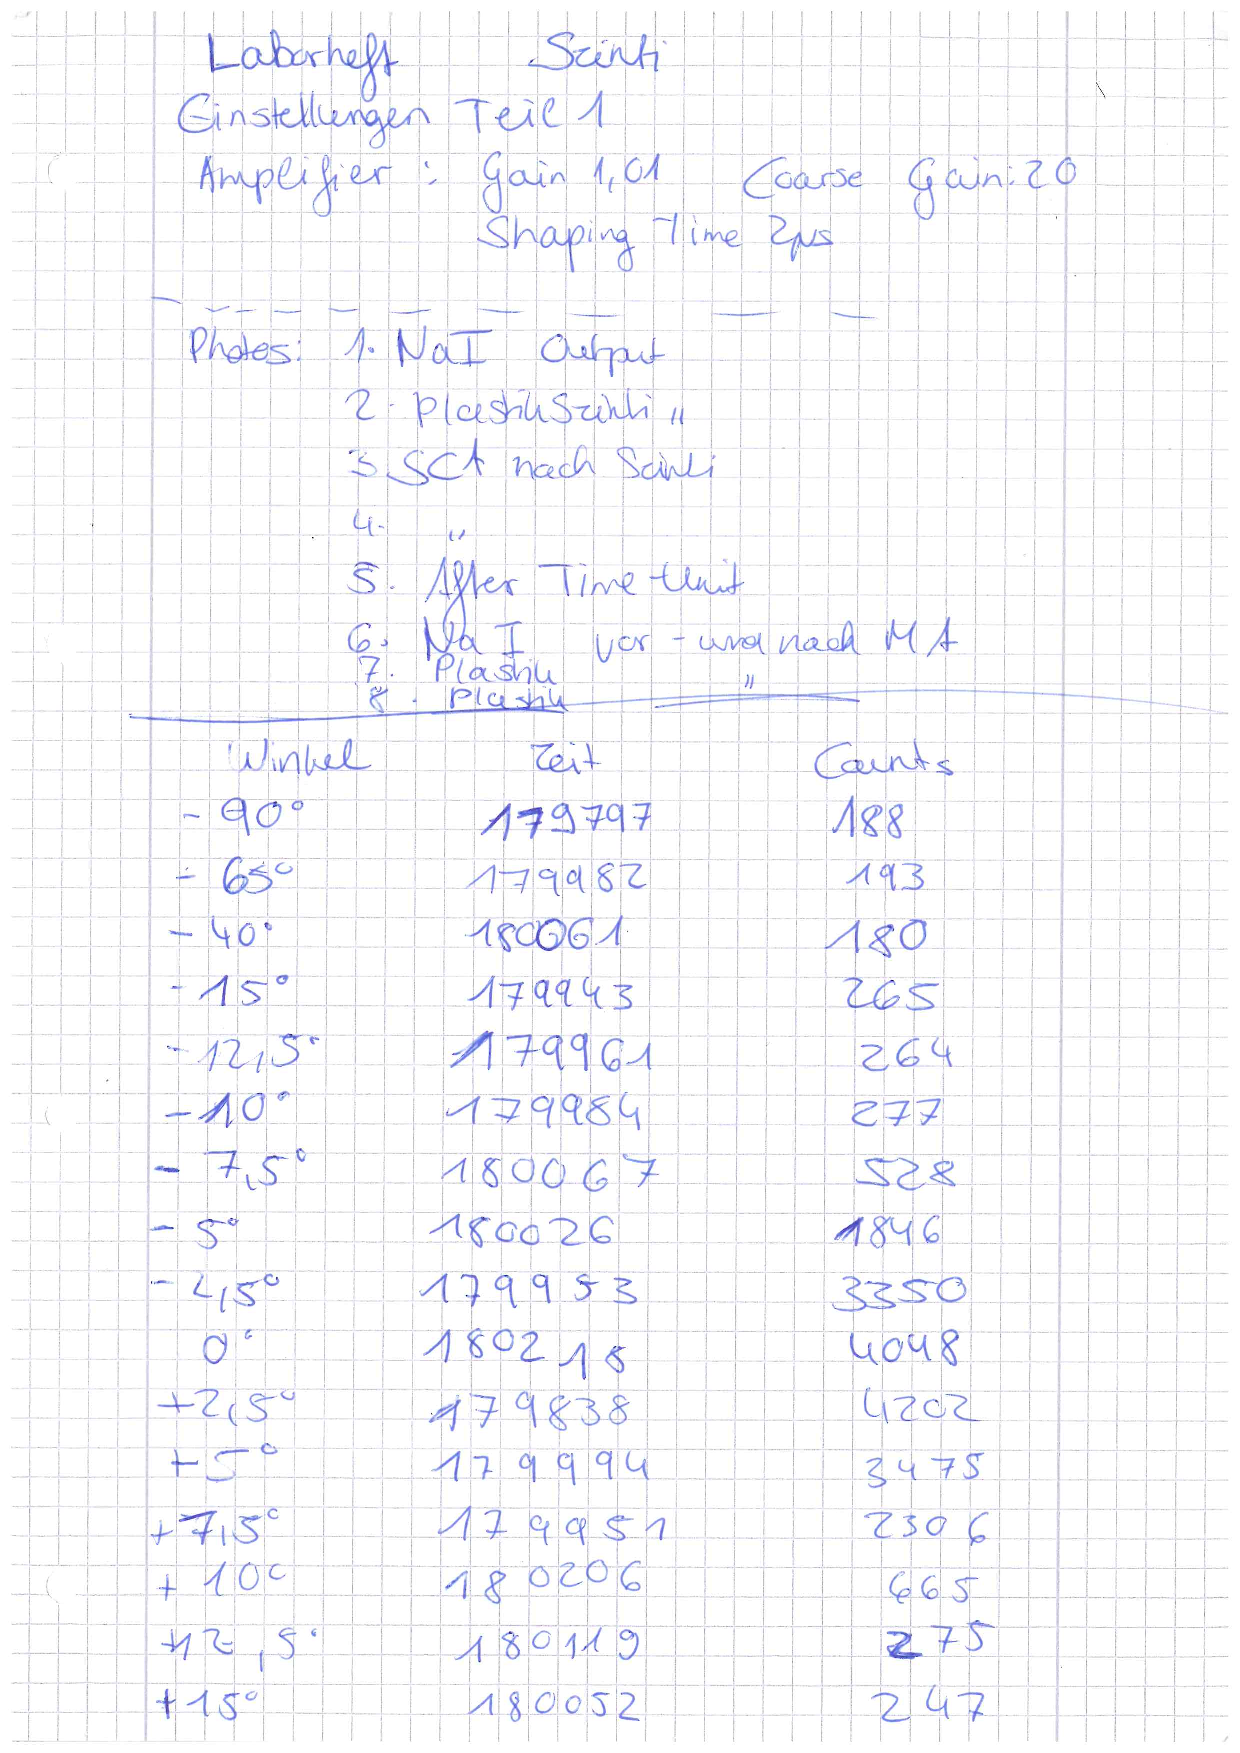
\includegraphics[width=0.9\textwidth]{figures/Laborheft1.pdf}
\end{minipage}
\newpage
\begin{minipage}{\textwidth}
	\centering
	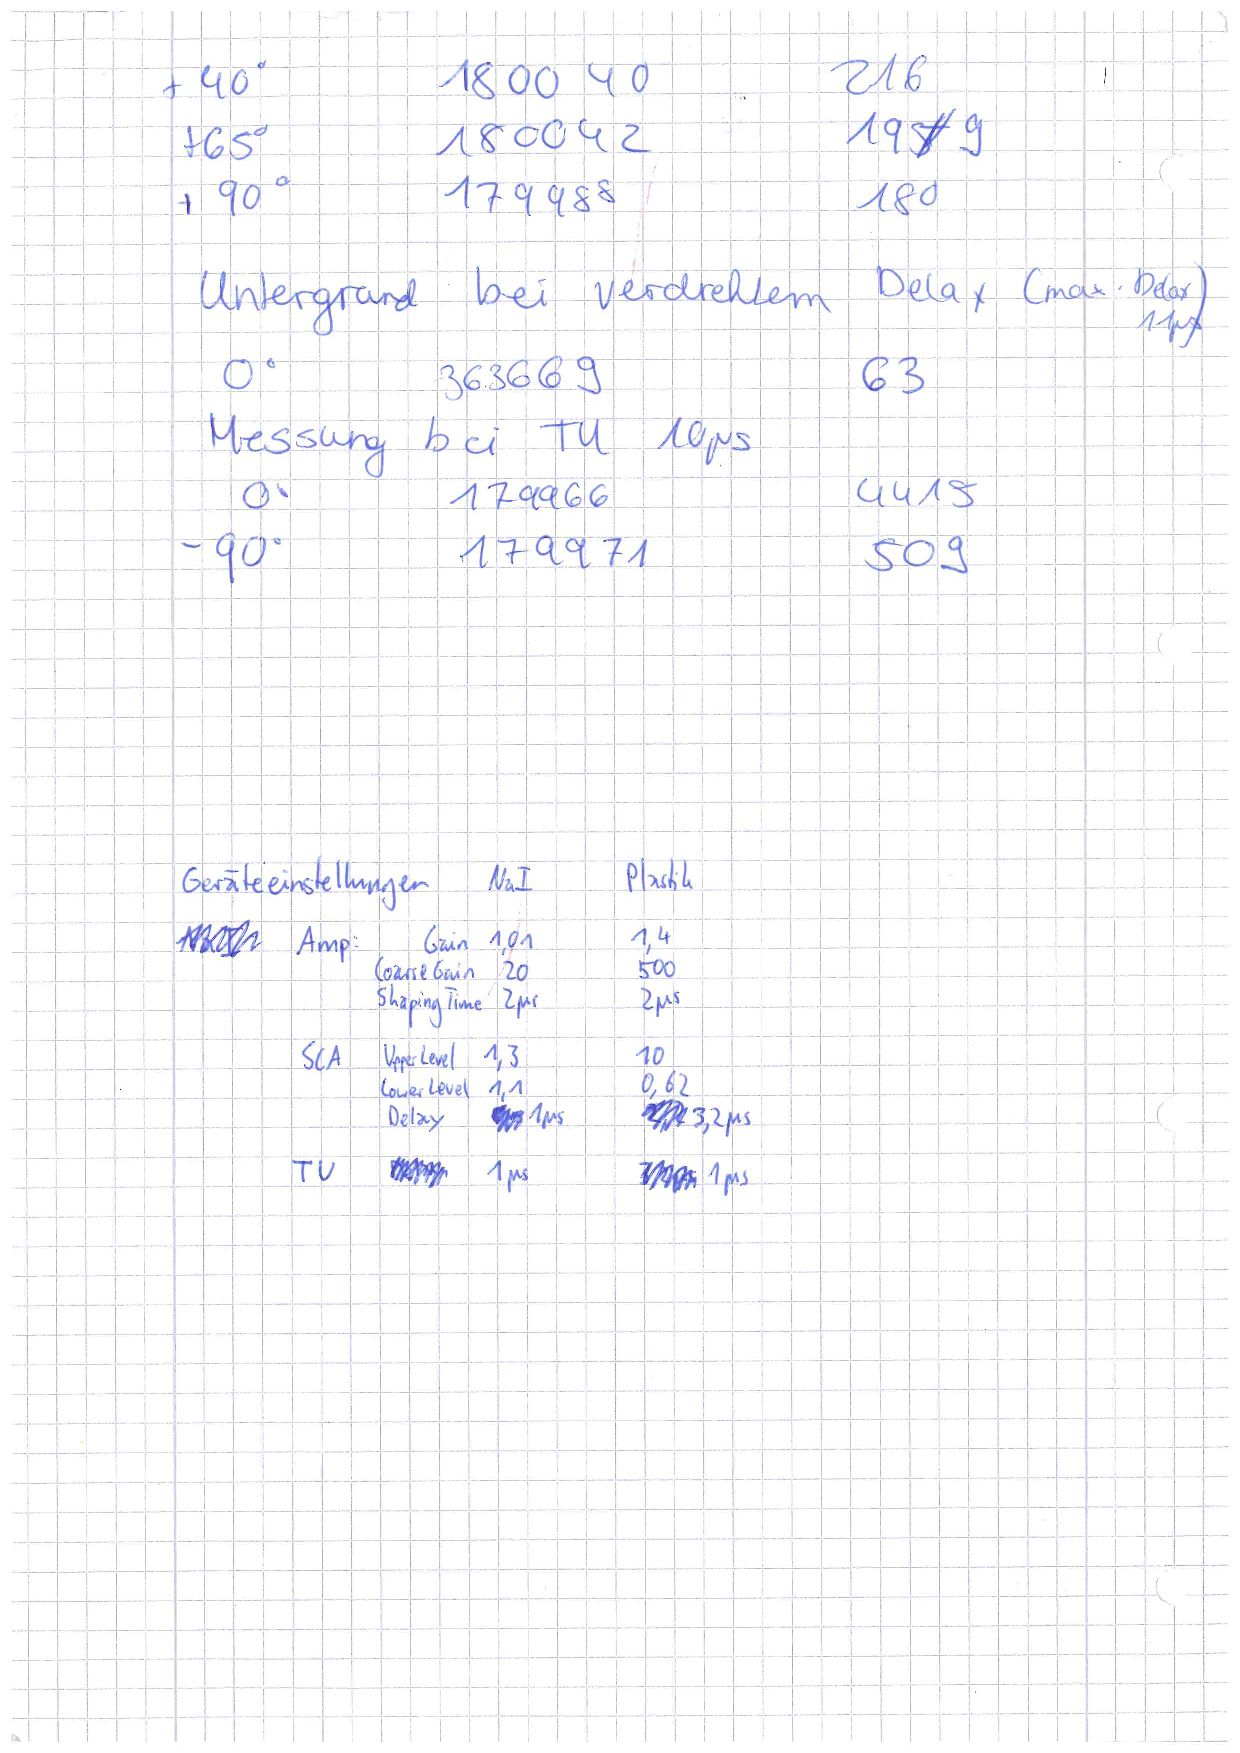
\includegraphics[width=0.9\textwidth]{figures/Laborheft2.pdf}
\end{minipage}
\label{Laborbuch}
\newpage

\thispagestyle{empty}
\begin{thebibliography}{9}

\bibitem{anleitung}
	M. Köhli,
	\emph{Versuchsanleitung: Szintillationszähler},
	Institut für Mathematik und Physik,
	Albert-Ludwigs-universität,
	2011
\bibitem{staat}
	Tobijas Kotyk,
	\emph{Versuche zur Radioaktivität im Physikalischen Fortgeschrittenen Praktikum an der Albert-Ludwigs-Universität Freiburg},
	Institut für Mathematik und Physik,
	Albert-Ludwigs-universität,
	2011
\bibitem{med}
	Dirk Hünninger, Kieran Maher, uvm.,
	\emph{Physikalische Grundlagen der Nuklearmedizin},
	Wikibooks.org,
	2012
\bibitem{photo}
	\emph{Praktikum im DESY Zeuthen}
	https://www-zeuthen.desy.de/exps/physik\_begreifen/chris/\\Photomultiplier.html,
	Stand: 27.09.15
	
\bibitem{Demtröder}
Wolfgang Demtröder
 \emph{Experimentalphysik 4: Kern-, Teilchen-, und Astrophysik},
 Springer-Verlag,
 4. Auflage,
 2014
 
 \bibitem{staat1}
 Simon Amrein,
 \emph{Staatsexamensarbeit: Halbleiter und Halbleiterdetektoren},\\
 Albert-Ludwigs-Universität Freiburg,
 Physikalisches Institut,
 2008
 
\bibitem{energien1}
\emph{http://hacol13.physik.uni-freiburg.de/fp/Versuche/FP1/FP1-3-Szintillationszaehler/Anhang/Th-228\_tables.pdf}, Stand: 20.10.2016

\bibitem{energien2}
\emph{http://www.nucleide.org/DDEP\_WG/Nuclides/K-40\_tables.pdf}, Stand: 22.10.2016

\bibitem{energien3}
\emph{http://www.nucleide.org/DDEP\_WG/Nuclides/Cu-61\_tables.pdf}, Stand: 22.10.2016

\bibitem{anleitung1}
(Zerfall von $^{57}$Co): http://hacol13.physik.uni-freiburg.de/fp/Versuche/FP1/FP1-6-KurzeHalbwertzeiten/Anleitung.pdf
\end{thebibliography}

\end{document}